\documentclass[12pt]{article}
\usepackage{polski}
\usepackage[utf8]{inputenc}
\usepackage{amsfonts}
\usepackage{amsmath}
\usepackage{enumitem}
\usepackage{graphicx}
\setlength{\parskip}{1em}


\begin{document}
	\title{Sprawozdanie\\Metody Numeryczne 2, laboratorium 1}
	\author{Grzegorz Rozdzialik (D4, grupa lab. 2)}
	\maketitle	
	
	\section{Zadanie}
	{\Large Temat \textbf{2}, zadanie \textbf{49}:}\\
	Interpolacja funkcjami liniowymi na kwadracie podzielonym na $2n^2$ trójkątów przystających. Zagęszczanie podziału kwadratu, aż do osiągnięcia błędu średniokwadratowego, mierzonego w środkach ciężkości trójkątów, mniejszego od $\varepsilon$.
	
	Mając funkcję interpolowaną $f: D \to \mathbb{R}$, gdzie $D = \{ (x, y) \in \mathbb{R}^2: x_0 \leq x \leq x_0 + H, y_0 \leq y \leq y_0 + H\}$, $H, x_0, y_0 \in \mathbb{R}$ opisaaną na kwadracie o boku $H$, którego lewy dolny wierzchołek ma współrzędne $(x_0, y_0)$, należy skonstruować funkcję sklejaną złożoną z funkcji opisanych na pojedynczych trójkątach przystających, dzielących ten kwadrat.
	
	\begin{figure}[]
		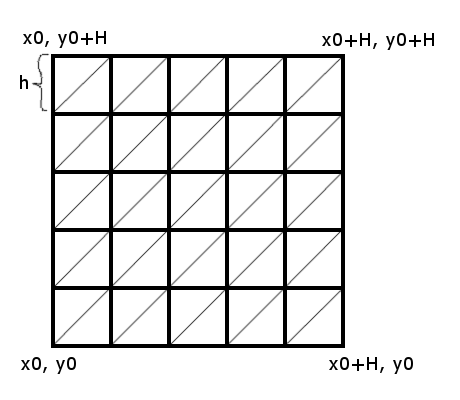
\includegraphics[scale=0.8]{square-division.png}
		\caption{Przedstawienie podziału dziedziny funkcji $f$}
	\end{figure}

	Dziedzinę funkcji $f$ należy podzielić na $n$ części wzdłuż osi $x$ oraz osi $y$, co daje $n^2$ kwadratów, a następnie każdy kwadrat można podzielić względem dowolnej przekątnej. W moim rozwiązaniu użyłem przekątnej o współczynniku kierunkowym równym $1$.
	
	\section{
	
\end{document}